\documentclass[12pt]{article}
\usepackage[a4paper, margin=0.75in]{geometry}
\usepackage[document]{ragged2e}
\usepackage{graphicx}
\usepackage{placeins}
\graphicspath{ {./images/} }
\usepackage{enumerate}
\usepackage{framed}
\usepackage{amsmath,amsfonts,amsthm,thmtools,amssymb,mathtools,commath}
\usepackage{physics}
\usepackage{tikz}
\usetikzlibrary{mindmap}
\usepackage{caption}
\usepackage{xcolor}
\usepackage[most]{tcolorbox}
\usepackage{cleveref}


%%%%%%%%%%%%%%%%
%  Definition  %
%%%%%%%%%%%%%%%%
\tcbuselibrary{theorems,skins,hooks}
\newtcbtheorem[number within=subsection]{definition}{Definition}%
{
    % theorem style=definition,
    enhanced,
	before skip=2mm,after skip=2mm, colback=cyan!5,colframe=cyan!80!black,boxrule=0.5mm,
	attach boxed title to top left={xshift=1cm,yshift*=1mm-\tcboxedtitleheight},
	boxed title style={frame code={
					\path[fill=cyan]
					([yshift=-1mm,xshift=-1mm]frame.north west)
					arc[start angle=0,end angle=180,radius=1mm]
					([yshift=-1mm,xshift=1mm]frame.north east)
					arc[start angle=180,end angle=0,radius=1mm];
					\path[left color=cyan!30!black,right color=cyan!30!black,
						middle color=cyan!50!black]
					([xshift=-2mm]frame.north west) -- ([xshift=2mm]frame.north east)
					[rounded corners=1mm]-- ([xshift=1mm,yshift=-1mm]frame.north east)
					-- (frame.south east) -- (frame.south west)
					-- ([xshift=-1mm,yshift=-1mm]frame.north west)
					[sharp corners]-- cycle;
				},interior engine=empty,
		},
	fonttitle=\bfseries,
	title={#2},#1
}{def}


%%%%%%%%%%%%%
%  Theorem  %
%%%%%%%%%%%%%
\tcbuselibrary{theorems,skins,hooks}
\newtcbtheorem[use counter from=definition]{theorem}{Theorem}%
{
    theorem style=plain,
    enhanced,
    colframe=green,
    boxrule=1pt,
    titlerule=0mm,
    toptitle=1mm,
    bottomtitle=1mm,
    fonttitle=\bfseries,
    fontupper=\mdseries\itshape,
    coltitle=green!30!black,
    colbacktitle=cyan!15!white,
    colback=green!10,
    description font=\bfseries\sffamily
}{thrm}


%%%%%%%%%%%%%%
% Corollary  %
%%%%%%%%%%%%%%
 \tcbuselibrary{theorems,skins}
 \newtcbtheorem[use counter from=theorem]{corollary}{Corollary}%
 {
    theorem style=plain,
    enhanced,
    colframe=green,
    frame hidden,
    titlerule=0mm,
    toptitle=1mm,
    bottomtitle=1mm,
    fonttitle=\bfseries,
    fontupper=\mdseries\itshape,
    coltitle=green!30!black,
    colbacktitle=cyan!15!white,
    colback=green!10,
    description font=\bfseries\sffamily
 }{corl}


%%%%%%%%%%%%%
%  Example  %
%%%%%%%%%%%%%
\tcbuselibrary{theorems,skins,hooks}
\newtcbtheorem[number within=section]{example}{Example}%
{
	enhanced,
	breakable,
	colback = gray!5,
	frame hidden,
	boxrule = 0sp,
	borderline west = {2pt}{0pt}{gray},
	sharp corners,
	detach title,
	before upper = \tcbtitle\par\smallskip,
    coltitle=gray!70!black,
	fonttitle = \bfseries\sffamily,
	description font = \mdseries\bfseries
}
{xmp}


%%%%%%%%%%%%%%
%  Exercise  %
%%%%%%%%%%%%%%
\tcbuselibrary{theorems,skins,hooks}
\newtcbtheorem[number within=section]{exercise}{Exercise}%
{
    enhanced,
    breakable,
    colback=black!5,
    colframe=black!30,
    left=0.5em,
    before skip=10pt,
    after skip=10pt,
    boxrule=0pt,
    boxsep=0pt,
    arc=0pt,
    outer arc=0pt,
    borderline west={3pt}{0pt}{black!30},
}{exc}

%%%%%%%%%%
%  Note  %
%%%%%%%%%%
\usetikzlibrary{arrows,calc,shadows.blur}
\tcbuselibrary{skins}
\newtcolorbox{note}[1][]{%
	enhanced jigsaw,
	colback=gray!20!white,%
	colframe=gray!80!black,
	size=small,
	boxrule=1pt,
	title=\textbf{Note:-},
	halign title=flush center,
	coltitle=black,
	breakable,
	drop shadow=black!50!white,
	attach boxed title to top left={xshift=1cm,yshift=-\tcboxedtitleheight/2,yshifttext=-\tcboxedtitleheight/2},
	minipage boxed title=1.5cm,
	boxed title style={%
			colback=white,
			size=fbox,
			boxrule=1pt,
			boxsep=2pt,
			underlay={%
					\coordinate (dotA) at ($(interior.west) + (-0.5pt,0)$);
					\coordinate (dotB) at ($(interior.east) + (0.5pt,0)$);
					\begin{scope}
						\clip (interior.north west) rectangle ([xshift=3ex]interior.east);
						\filldraw [white, blur shadow={shadow opacity=60, shadow yshift=-.75ex}, rounded corners=2pt] (interior.north west) rectangle (interior.south east);
					\end{scope}
					\begin{scope}[gray!80!black]
						\fill (dotA) circle (2pt);
						\fill (dotB) circle (2pt);
					\end{scope}
				},
		},
	#1,
}


\title{
    CSE-284: Object Oriented Programming \\
    Experiment 2: Constructor and Destruction in OOP
}

\author{
    Turja Roy \\ 
    ID: 2108052 \\ 
    Group: G-2
}
\date{}

\begin{document}
\maketitle

\section*{Objectives:}
\begin{itemize}
    \item Introduction with Constructor class in C++.
    \item To define different types of constructors.
    \item To learn Constructor and Destructor in C++.
\end{itemize}


\FloatBarrier
\section*{Example 1}
Write a C++ program to demonstrate the use of the default constructor.

\subsection*{Code}
\lstinputlisting[language=C++]{../Exp-1.cpp}

\subsection*{Output}
\vspace{-1em}
\begin{figure}[htpb]
    \centering
    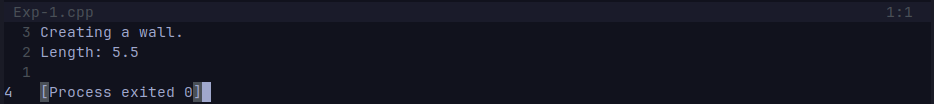
\includegraphics[width=0.7\textwidth]{Exp-1.png}
    \caption{Output of Exp-1.cpp}
\end{figure}


\FloatBarrier
\section*{Example 2}
Write a C++ program to demonstrate the use of Parameterized Constructor.

\subsection*{Code}
\lstinputlisting[language=C++]{../Exp-2.cpp}

\subsection*{Output}
\begin{figure}[htpb]
    \centering
    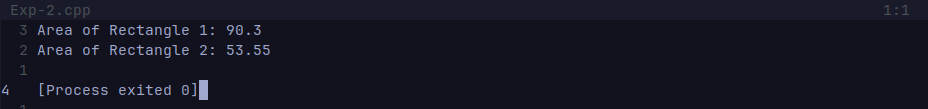
\includegraphics[width=0.8\textwidth]{Exp-2.png}
    \caption{Output of Exp-2.cpp}
\end{figure}


\FloatBarrier
\section*{Example 3}
Write a C++ program to demonstrate the use of Copy Constructor.

\subsection*{Code}
\lstinputlisting[language=C++]{../Exp-3.cpp}

\subsection*{Output}
\begin{figure}[htpb]
    \centering
    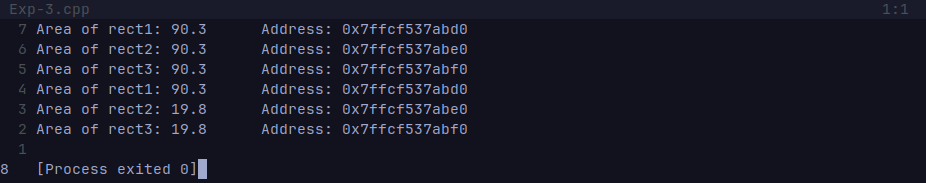
\includegraphics[width=0.8\textwidth]{Exp-3.png}
    \caption{Output of Exp-3.cpp}
\end{figure}


\FloatBarrier
\section*{Example 4}
Write a C++ program to understand the Destructor Class in C++.

\subsection*{Code}
\lstinputlisting[language=C++]{../Exp-4.cpp}

\subsection*{Output}
\begin{figure}[htpb]
    \centering
    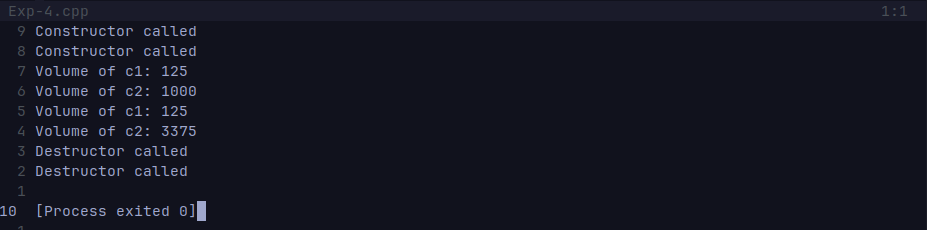
\includegraphics[width=0.7\textwidth]{Exp-4.png}
    \caption{Output of Exp-4.cpp}
\end{figure}


\FloatBarrier
\section*{Lab Task}
Write a C++ program with a class named \texttt{Student} that contains three variables \texttt{a, b, c}. If a constructor is not used, the variables will be initialized with values \texttt{1, 2, 3} respectively. If a constructor is used, the variables will be initialized with the values passed as arguments.

\subsection*{Code}
\lstinputlisting[language=C++]{../Lab-Test.cpp}


\FloatBarrier
\section*{Practice 1}
Suppose you have a Savings Account with an initial amount of 500 and you have to add some more amount to it. Create a class 'AddMoney' with a data member named 'amount' with an initial value of 500. Now make two constructors of this cclass as follows:
\begin{itemize}
    \item without any parameter -- no amount will be added to the Savings Account. 
    \item having a parameter which is the amount that will be added to the Savings Account.
\end{itemize}
Create an object of the 'AddMoney' class and display the final amount in the Savings Account.

\subsection*{Code}
\lstinputlisting[language=C++]{../Prac-1.cpp}

\subsection*{Output}
\begin{figure}[htpb]
    \centering
    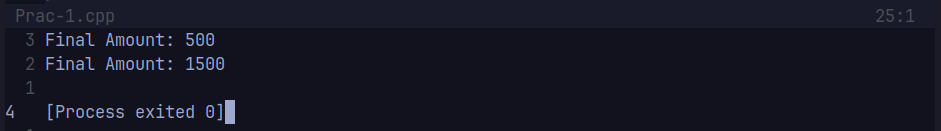
\includegraphics[width=0.7\textwidth]{Prac-1.png}
    \caption{Output of Prac-1.cpp}
\end{figure}


\FloatBarrier
\section*{Practice 2}
Write a C++ program to define a class 'Car' with the following specifications:
\begin{itemize}
    \item Private members:
        \begin{itemize}
            \item \texttt{car\_name}, \texttt{model\_name}, \texttt{fuel\_type}: string type 
            \item \texttt{mileage}: float type 
            \item \texttt{price}: float type
        \end{itemize}
    \item Public members:
        \begin{itemize}
            \item \texttt{displaydata()}: Function to display the data members on the screen.
        \end{itemize}
\end{itemize}
Use Constructor (both Default and parameterized) and Destructor. When no parameter is passed, the default Constructor will be called with the message "Default Constructor has been called."

\subsection*{Code}
\lstinputlisting[language=C++]{../Prac-2.cpp}

\subsection*{Output}
\begin{figure}[htpb]
    \centering
    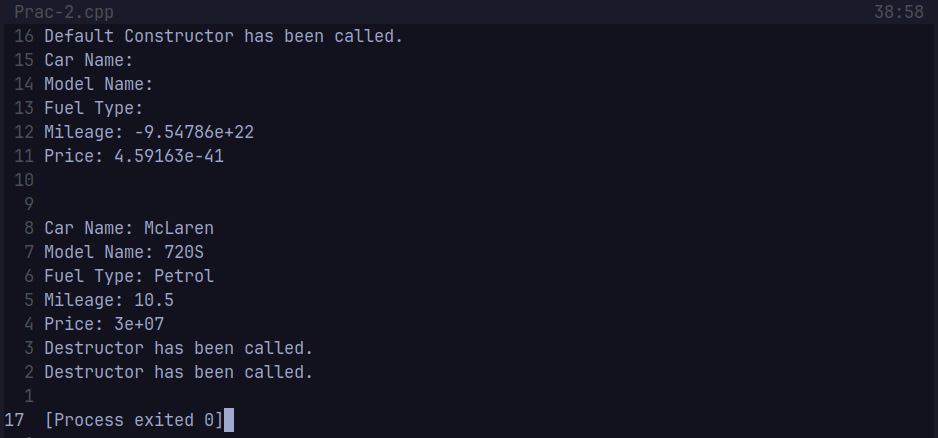
\includegraphics[width=0.8\textwidth]{Prac-2.png}
    \caption{Output of Prac-2.cpp}
\end{figure}


\newpage
\section*{Discussion}
\begin{itemize}
    \item In this lab, constructors and destructors were discussed.
    \item Default and parameterized constructors were implemented. 
    \item In experiment 3, the copy constructor was used to copy the values of one object to another object. 
    \item While using copy constructor, the addresses were checked. It can be noticed that the addresses of the two objects were different even though the values were the same. 
    \item The destructor is always called at the end of the program. It is used to free the memory allocated to the object. 
    \item When calling the default constructor, if no value is assigned for the variables, garbage values are assigned there.
\end{itemize}

\end{document}
